\section{Index Construction}
\label{preprocessing}


As the decentralized search relies on the index structure to find paths, the constructed indexes serve as a crucial factor for accurate approximations. Previous works have studied various landmark selection strategies which have a significant impact on the accuracy of online query. In our study, we observe that even with the same landmark set, choosing which edges to be indexed also has a great impact on the accuracy of online search. Because in practical networks, it is very common that there are more than one shortest paths from a vertex to a landmark. Furthermore, each vertex only stores one shortest path in their labels for each landmark. Different shortest paths indicate that different edges are indexed. In this section, we discuss how this will effect the accuracy of online search and propose a heuristic index construction algorithm that can generate an index more suitable for decentralized searches in terms of online query accuracy.


\begin{figure}[t]
    \centering
    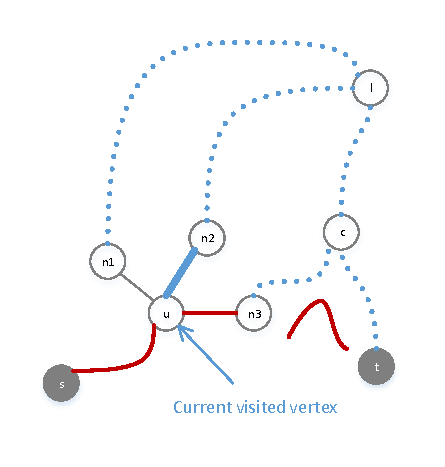
\includegraphics[width=\linewidth]{../figures/new_illustrate/vis_dec.pdf}
    \caption{Decentralized search selects vertices with lowest common ancestor with target vertex at each step.}
    \label{fig:vis_dec}
\end{figure}

\begin{figure*}[htbp]
    \centering
    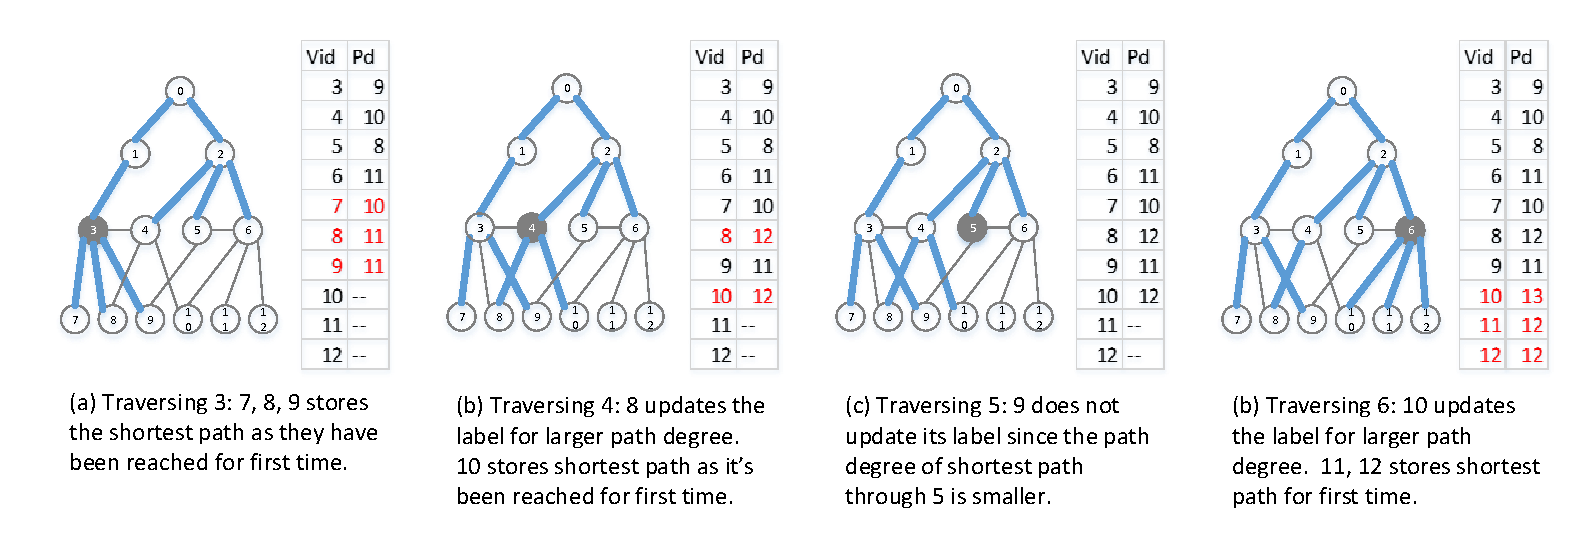
\includegraphics[width=\linewidth]{../figures/new_illustrate/bfs_illustrate.pdf}
    \caption{Heuristic algorithm that index shortest path with highest path degree during breadth first search}
    \label{fig:bfs_illustrate}
\end{figure*}

\subsection{Impact of index on query accuracy}
Although all shortest paths between two vertices are equivalent in terms of lengths, it is not necessary that they have same impact on the decentralized search since they have different vertices along the paths. Recall that in decentralized searches, at each step, the search will traverse neighbors of the currently visited vertex to find one with the shortest LCA distance to the target. Hence, a common ancestor means that the indexed shortest paths of two vertices intersect with each other. By doing this, decentralized search actually finds the neighbor with indexed shortest path that has an intersection with the indexed shortest path of target vertex at a lower level than other neighbors and the current visited vertex. For example, in Fig. \ref{fig:vis_dec}, the dotted line shows indexed shortest paths to the landmark with vertices along the path. When examining edges adjacent to $u$, $n_3$ will be chosen as the next step due to that it has a lower common ancestor $c$ than the other neighbors and $u$. Note that all the neighbors will have a common ancestor at the root with the target vertex as long as they are in the same connected component. But such common ancestors will not lead to a shorter path, so we do not need to consider them in our algorithm.

For a certain vertex $u$, it is possible to find the best shortest path from landmark to be indexed so that the shortest approximate path can be found from one vertex $v$ to $u$. But such a shortest path may lead to a longer approximate path from another vertex $w$ to $u$. The case will be much more complex when considering all the other vertices in the whole graph. So when constructing label for each vertex, we need to think about average cases. For each vertex, we want to find a shortest path to be indexed that has common ancestors with a larger number of other vertices. This is because during the decentralized search, the more neighbors of current visited vertex has common ancestor with target vertex, the higher the chance there will be a common ancestor at a lower level which suggests a shorter path. As we discussed before, a common ancestor means that two paths have intersections. So we are actually looking for the shortest path which intersects with most other paths to increase the chance for decentralized search to find a shorter path from other vertices to this one.

\subsection{Heuristic index construction algorithm}

We propose a greedy heuristic to construct an index which can lead to better accuracy in online queries. For each vertex  $u$, when generating a label for it to store a shortest path to landmark $l$, as we discussed above, among all the shortest paths we want to store the one that intersects with most other paths. But it will be quite costly to calculate the number of paths a shortest path intersect with. To achieve this goal, we use a value which is much easier to compute to compare different shortest paths, the degree of all the vertices along each shortest path. We call this value the path degree $Pd$. The intuition here is that the higher the path degree of a path, the more other paths it may intersect with. Path degree can be easily calculated by summing up the degree of vertices along the path.

Same as the shortest path, the path degree of shortest path also follows optimal substructure. That is, if $(u, .., w, ..., v)$ has the highest path degree among all the shortest path from $u$ to $v$, then the path degree of $(u, ..., w)$ is also the highest among all the shortest path from $u$ to $w$. So for each vertex, the shortest path with highest degrees can be calculated easily by comparing path degree of indexed shortest path of its parents and selecting the highest one. Such calculation can be done during breadth first search with little overhead by caching the path degree of the label of each vertex. Fig. \ref{fig:bfs_illustrate} shows an example of how to greedily select shortest path with the highest path degree during breadth first search. When traversing vertex $4$, even though vertex $8$ has already been indexed with a shortest path $(0, 1, 3, 8)$ into its label, due to that $(0, 2, 4, 8)$ has a higher path degree, the label of vertex $8$ is updated. The same thing happens to vertex $10$ while traversing vertex $6$.

%
%To see which way to do the Breadth First Search may construct a better quality index, we need to look at what is effect the quality of index. LCA distance is the only criterion used by decentralized search. And the LCA distance is determined by the least common ancestor that has been embedded into the label of both vertex. Clearly, due to the limited size of indexes, for an arbitrary pair of vertices, it is possible that the least common ancestor suggested by the index is not the lowest one of the underlying graph. For example in Fig.\ref{fig:single_level} for index scheme 1, vertex $6$ and $9$ have least common ancestor $1$ in the underlying graph, yet it is possible to extract this common ancestor with index scheme 1. Although it is almost impossible to embed the lowest possible least common ancestor for all pairs of vertices in the index. The performance we care about is the average performance, which means we only need to find a strategy that can embed lower least common ancestors for more pairs of vertices. Then the average approximation error could be reduced. For example in Fig.\ref{fig:single_level}, with the same underlying graph, different ways to build the shortest path tree index cause different number of pairs of vertices cannot retrieve their exact distance from the index because the LCA computed by the index is not actually the lowest one in the underlying graph. The more pairs of vertices have a lower LCA, the better performance the index will have during online query.
%
%Let's first see one level from level structure of Breadth First Search tree. Assuming all vertices at level $k$ have already been pushed to the queue. The question is among all the edges from vertices in level $k$ to vertices in level $k+1$, which of them should be embedded into the index. Or an equal question is among all the parent vertex in level $k$ of a vertex $v$ in level $k+1$ has, which one should be embedded into the label of vertex $v$. For vertices in level $k+1$, if they both embed a same vertex $u$ in level $k$ to their label, then vertex $u$ is their least common ancestor at lowest possible level. Since an edge that has both ends in same level will never happen in the shortest path indexes. For pairs of vertices that one is in level $k$ and the other one is in level $k+1$, if the one in level $k$ is in the label of the other one, then it is also their least common ancestor at lowest possible level. Intuitively, if we want build an index that incorporate LCA at lowest possible level for more pairs of vertices, high degree vertices should be preferred than low degree vertices. For example in Fig.\ref{fig:single_level}, the index scheme 1 have $8$ pairs of vertices that does not have their lCA at lowest possible level, while the index scheme 2 have $9$ pairs.
%
%\comment {TODO: how hard is is to find an optimal index}
%While finding the optimal index usually require too much overheads for an approximation algorithm like this, simple heuristic algorithms can be used without sacrificing the performance a lot. For example for a greedy algorithm, at level $k+1$, it simply embed the edge with highest degree parent at level $k$ to its label.
%\comment {TODO: how good is greedy algorithm, or why is it good for practical graphs}
%
%\subsection{Optimize for multiple level}
%

%
%In the last section we have discussed about optimizing index for a single level from the level structure of Breadth First Search tree. But simply doing optimizing for each level does not guarantee the overall optimality. For example in Fig.\ref{fig:multi_level}, the index scheme 1 is optimized by the single level greedy heuristic, however, the overall index does not outperform the index scheme 2. The reason that algorithms works on a single level does not work so well on the graph is that it could be the case that a high degree vertex does not have high degree parents. Clearly, finding an optimal index for the whole graph is a much harder problem than the single level case, so we will also consider heuristic algorithms.
%
%In single level problem, the high degree heuristic works pretty well because a higher degree suggest more pairs of vertices have their LCA at lowest possible level. When the problem is extended from a single level to the whole graph, for each vertex, we could also use the same heuristic. Among all the possible shortest path from each vertex to the root, we want to find the one that have LCA at lower level with most other vertices. Not that for a specific shortest path, as long as any other vertices have a part of this path in their label, they will have a LCA at a lower level than the root. All the other vertices that does not include any part of this path except the root, which all the label contains, will have the LCA at the root. So instead of choosing the path with highest degree of direct parent vertex, the algorithm should add the degree of all vertices along the path and pick the one with highest total value. Similar to the heuristic algorithm for single level, such a heuristic algorithms have the same and storage complexity with regular BFS.



